\subsection{Misure ad angolo $<\SI{90}\degree$}

\begin{figure}
	% \vspace{-1.5cm}
	\hspace{-0.25\textwidth}
	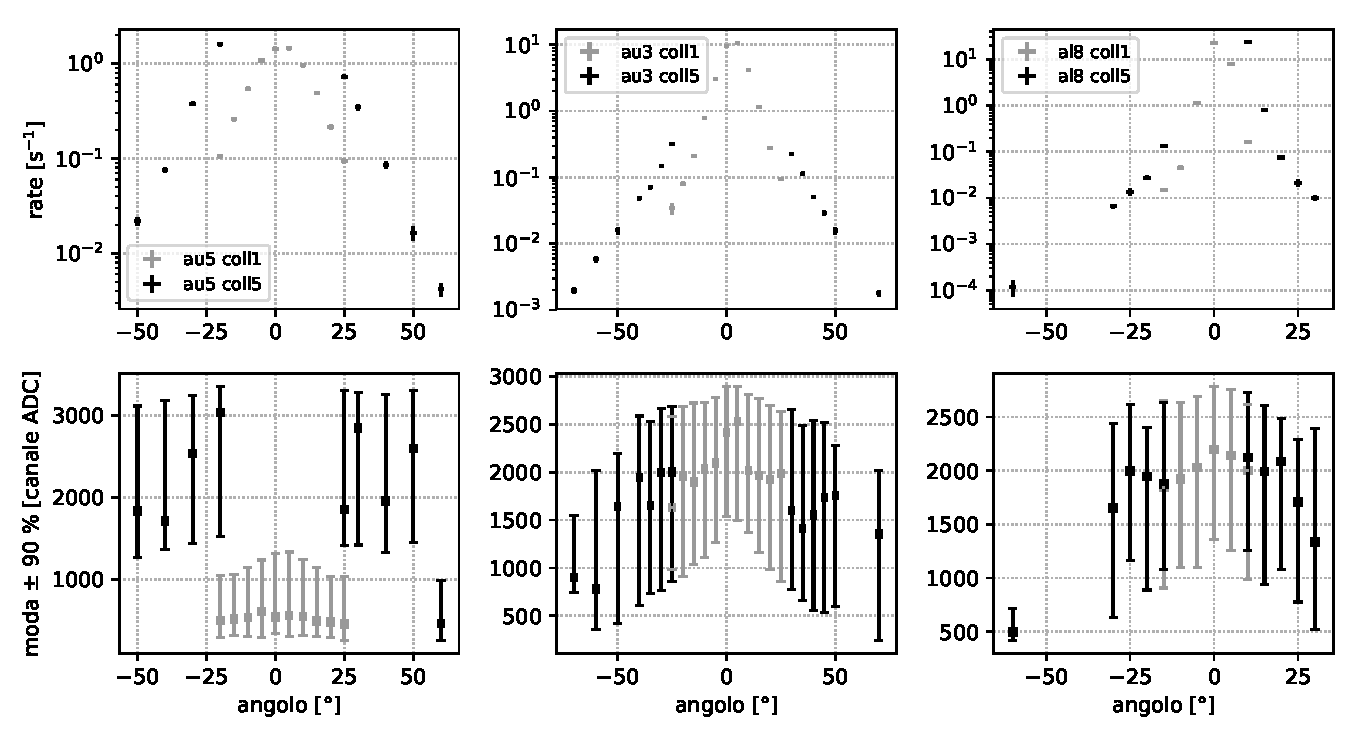
\includegraphics[width=1.5\textwidth]{immagini/spettri}
	\caption{\label{fig:spettri}
	Misure di rate per angoli minori di \SI{90}\degree.
	Gli spettri sono riportati come la moda con una barra
	che contiene il \SI{90}\% dello spettro a densità maggiore
	(la moda e la densità sono calcolate con una KDE).
	La legenda usa il formato \texttt{<elemento><spessore [\si{\micro m}]> coll<larghezza collimatore [\si{mm}]>}.
	Per l'oro da \SI5{\micro m} gli spettri con collimatore \SI5{mm}
	sono presi con guadagno dell'amplificatore 200,
	in tutti gli altri casi il guadagno è 50.}
\end{figure}

Abbiamo eseguito le misure di rate al variare dell'angolo
con le lamine di oro da \SI{3}{\micro m} e \SI5{\micro m} e con quella di alluminio da \SI8{\micro m},
sia con il collimatore da \SI1{mm} che da \SI5{mm}.
In tutte le misure abbiamo salvato lo spettro.
Le misure sono riportate in \autoref{fig:spettri}.
Gli eventi taggati come rumore risultano sempre minori dell'incertezza sul conteggio.
Per ogni configurazione la camera è rimasta chiusa durante tutta la serie di misure,
quindi l'eventuale disallineamento dell'angolo è lo stesso.
Fa eccezione la presa dati oro \SI{5}{\micro m} collimatore \SI5{mm} per la quale
le misure per $|\theta| \le \SI{30}{\degree}$ soddisfano il requisito
mentre le misure agli altri angoli sono inframezzate dall'apertura della camera e dal rimontaggio dell'apparato.
